\documentclass{standalone}
\usepackage{tikz}
\usetikzlibrary{calc}
\tikzset{%
  add/.style args={#1 and #2}{
    to path={%
      ($(\tikztostart)!-#1!(\tikztotarget)$)--($(\tikztotarget)!-#2!(\tikztostart)$)%
      \tikztonodes},add/.default={.2 and .2}}
}


\tikzset{%
  mark coordinate/.style={inner sep=0pt,outer sep=0pt,minimum size=2pt,
    fill=black,circle}%
}

\newcommand\pgfmathsinandcos[3]{%
  \pgfmathsetmacro#1{sin(#3)}%
  \pgfmathsetmacro#2{cos(#3)}%
}
\newcommand\LongitudePlane[2][current plane]{%
  \pgfmathsinandcos\sinEl\cosEl{\Elevation} % elevation
  \pgfmathsinandcos\sint\cost{#2} % azimuth
  \tikzset{#1/.estyle={cm={\cost,\sint*\sinEl,0,\cosEl,(0,0)}}}
}
\newcommand\LatitudePlane[2][current plane]{%
  \pgfmathsinandcos\sinEl\cosEl{\Elevation} % elevation
  \pgfmathsinandcos\sint\cost{#2} % latitude
  \pgfmathsetmacro\ydelta{\cosEl*\sint}
  \tikzset{#1/.estyle={cm={\cost,0,0,\cost*\sinEl,(0,\ydelta)}}} %
}
\newcommand\DrawLongitudeCircle[1]{
  \LongitudePlane{#1}
  \tikzset{current plane/.prefix style={scale=\R}}
  \pgfmathsetmacro\angVis{atan(sin(#1)*cos(\Elevation)/sin(\Elevation))} %
  \draw[current plane, thin] (\angVis-180:1) arc (\angVis-180:\angVis:1);
  \draw[current plane, thick]  (\angVis:1) arc (\angVis:\angVis+180:1);
}%

\newcommand\DrawLArc[1]{
  \LongitudePlane{#1}
  \tikzset{current plane/.prefix style={scale=\R}}
  \pgfmathsetmacro\angVis{atan(sin(#1)*cos(\Elevation)/sin(\Elevation))} %
  \draw[current plane] (\angVis-180:1) arc (\angVis-180:\angVis:1);
  % \draw[current plane, thick]  (\angVis:1) arc (\angVis:\angVis+180:1);
}%

\newcommand\DrawLArcB[1]{
  \LongitudePlane{#1}
  \tikzset{current plane/.prefix style={scale=\R}}
  \pgfmathsetmacro\angVis{atan(sin(#1)*cos(\Elevation)/sin(\Elevation))} %
  % \draw[current plane, thin] (\angVis-180:1) arc (\angVis-180:\angVis:1);
  \draw[current plane]  (\angVis:1) arc (\angVis:\angVis+180:1);
}%

\newcommand\DrawPointOnSphere[3]{%
  \pgfmathsinandcos\sinLoM\cosLoM{#1}
  \pgfmathsinandcos\sinLaM\cosLaM{#2}
}


\begin{document}
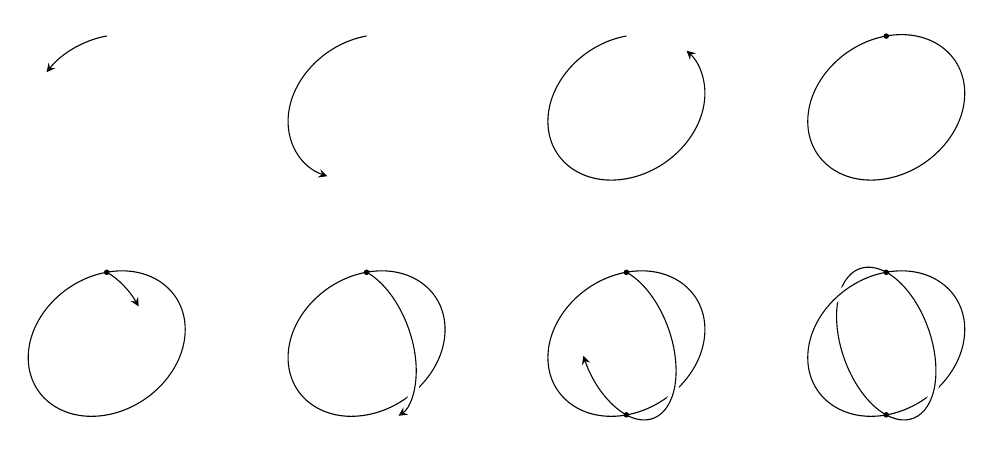
\begin{tikzpicture}[xscale=1.1]
  \def\R{1} % sphere radius
  \def\Elevation{25} % elevation angle
  \def\angleLongitudeP{-110} % longitude of point P
  \def\angleLongitudeQ{-45} % longitude of point Q
  \def\angleLatitudeQ{30} % latitude  Q    ; 0 latitude of P
  \def\angleLongitudeA{-20} % longitude of point A

  \pgfmathsetmacro\H{\R*cos(\Elevation)} % distance to north pole
  \LongitudePlane[PLongitudePlane]{\angleLongitudeP}
  \LongitudePlane[QLongitudePlane]{\angleLongitudeQ}
  \LongitudePlane[ALongitudePlane]{\angleLongitudeA}

  \coordinate (O) at (0,0);
  \coordinate[] (N) at (0,\H);
  \coordinate[] (S) at (0,-\H);

  \pgfmathsetmacro{\anglea}{25}
  \pgfmathsetmacro{\angleb}{125}

  \begin{scope}[xshift=-9cm]
    \LongitudePlane{\anglea}
    \tikzset{current plane/.prefix style={scale=\R}}
    \draw[current plane, -stealth] (90:1) arc (90:140:1);
  \end{scope}

  \begin{scope}[xshift=-6cm]
    \LongitudePlane{\anglea}
    \tikzset{current plane/.prefix style={scale=\R}}
    \draw[current plane, -stealth] (90:1) arc (90:240:1);
  \end{scope}

  \begin{scope}[xshift=-3cm]
    \LongitudePlane{\anglea}
    \tikzset{current plane/.prefix style={scale=\R}}
    \draw[current plane, -stealth] (90:1) arc (90:400:1);
  \end{scope}

  \begin{scope}
    \LongitudePlane{\anglea}
    \tikzset{current plane/.prefix style={scale=\R}}
    \draw[current plane] (90:1) arc (90:450:1);
    \coordinate[mark coordinate] () at (0,.25*3.62);
  \end{scope}

  \begin{scope}[xshift=-9cm, yshift=-3cm]
    \LongitudePlane{\anglea}
    \tikzset{current plane/.prefix style={scale=\R}}
    \draw[current plane] (90:1) arc (90:450:1);
    \coordinate[mark coordinate] () at (0,.25*3.62);

    \LongitudePlane{\angleb}
    \tikzset{current plane/.prefix style={scale=\R}}
    \draw[current plane, -stealth] (90:1) arc (90:130:1);
  \end{scope}

  \begin{scope}[xshift=-6cm, yshift=-3cm]
    \LongitudePlane{\anglea}
    \tikzset{current plane/.prefix style={scale=\R}}
    \draw[current plane] (90:1) arc (90:450:1);
    \coordinate[mark coordinate] () at (0,.25*3.62);

    \LongitudePlane{\angleb}
    \tikzset{current plane/.prefix style={scale=\R}}
    \draw[current plane, line width=3pt, white] (180:1) arc (180:210:1);
    \draw[current plane, -stealth] (90:1) arc (90:230:1);
  \end{scope}

  \begin{scope}[xshift=-3cm, yshift=-3cm]
    \LongitudePlane{\anglea}
    \tikzset{current plane/.prefix style={scale=\R}}
    \draw[current plane] (90:1) arc (90:450:1);
    \coordinate[mark coordinate] () at (0,.25*3.62);

    \LongitudePlane{\angleb}
    \tikzset{current plane/.prefix style={scale=\R}}
    \draw[current plane, line width=3pt, white] (180:1) arc (180:210:1);
    \draw[current plane, -stealth] (90:1) arc (90:330:1);
    \coordinate[mark coordinate] () at (0,-.25*3.62);
  \end{scope}

  \begin{scope}[yshift=-3cm]
    \LongitudePlane{\anglea}
    \tikzset{current plane/.prefix style={scale=\R}}
    \draw[current plane] (90:1) arc (90:450:1);
    \coordinate[mark coordinate] () at (0,.25*3.62);

    \LongitudePlane{\angleb}
    \tikzset{current plane/.prefix style={scale=\R}}
    \draw[current plane, line width=3pt, white] (180:1) arc (180:210:1);
    \draw[current plane] (90:1) arc (90:450:1);
    \coordinate[mark coordinate] () at (0,-.25*3.62);

    \LongitudePlane{\anglea}
    \tikzset{current plane/.prefix style={scale=\R}}
    \draw[current plane, white, line width=3pt] (110:1) arc (110:140:1);
    \draw[current plane] (110:1) arc (110:140:1);
  \end{scope}

\end{tikzpicture}

\end{document}
